%----------------------------------------------------------------------------------------
%	Section: Viewer Actions
%----------------------------------------------------------------------------------------
\section{Viewer Actions}

\begin{figure}[h]
    	\centering
    		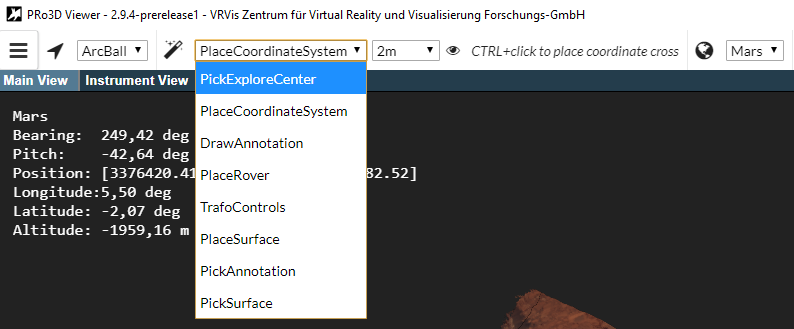
\includegraphics[width=1\textwidth]{pics/Interactions.png}
    	\caption[Interactions]{Viewer Actions.}
    	\label{fig:Interactions}
   \end{figure}

Once the surface is loaded there are different actions to choose (Figure~\ref{fig:Interactions}).
%----------------------------------------------------------------------------------------
%	SubSection: Pick Explore Center
%----------------------------------------------------------------------------------------
\subsection{Pick Explore Center}
\label{sec:pickEC}

The ``PickExploreCenter'' action concerns the \textbf{ArcBall} navigation mode. There are two navigation modes (Figure~\ref{fig:exploreCenter}):
\begin{itemize}
	\item \textbf{FreeFly} and 
	\item \textbf{ArcBall}.
\end{itemize}

\begin{figure}[h]
    	\centering
    		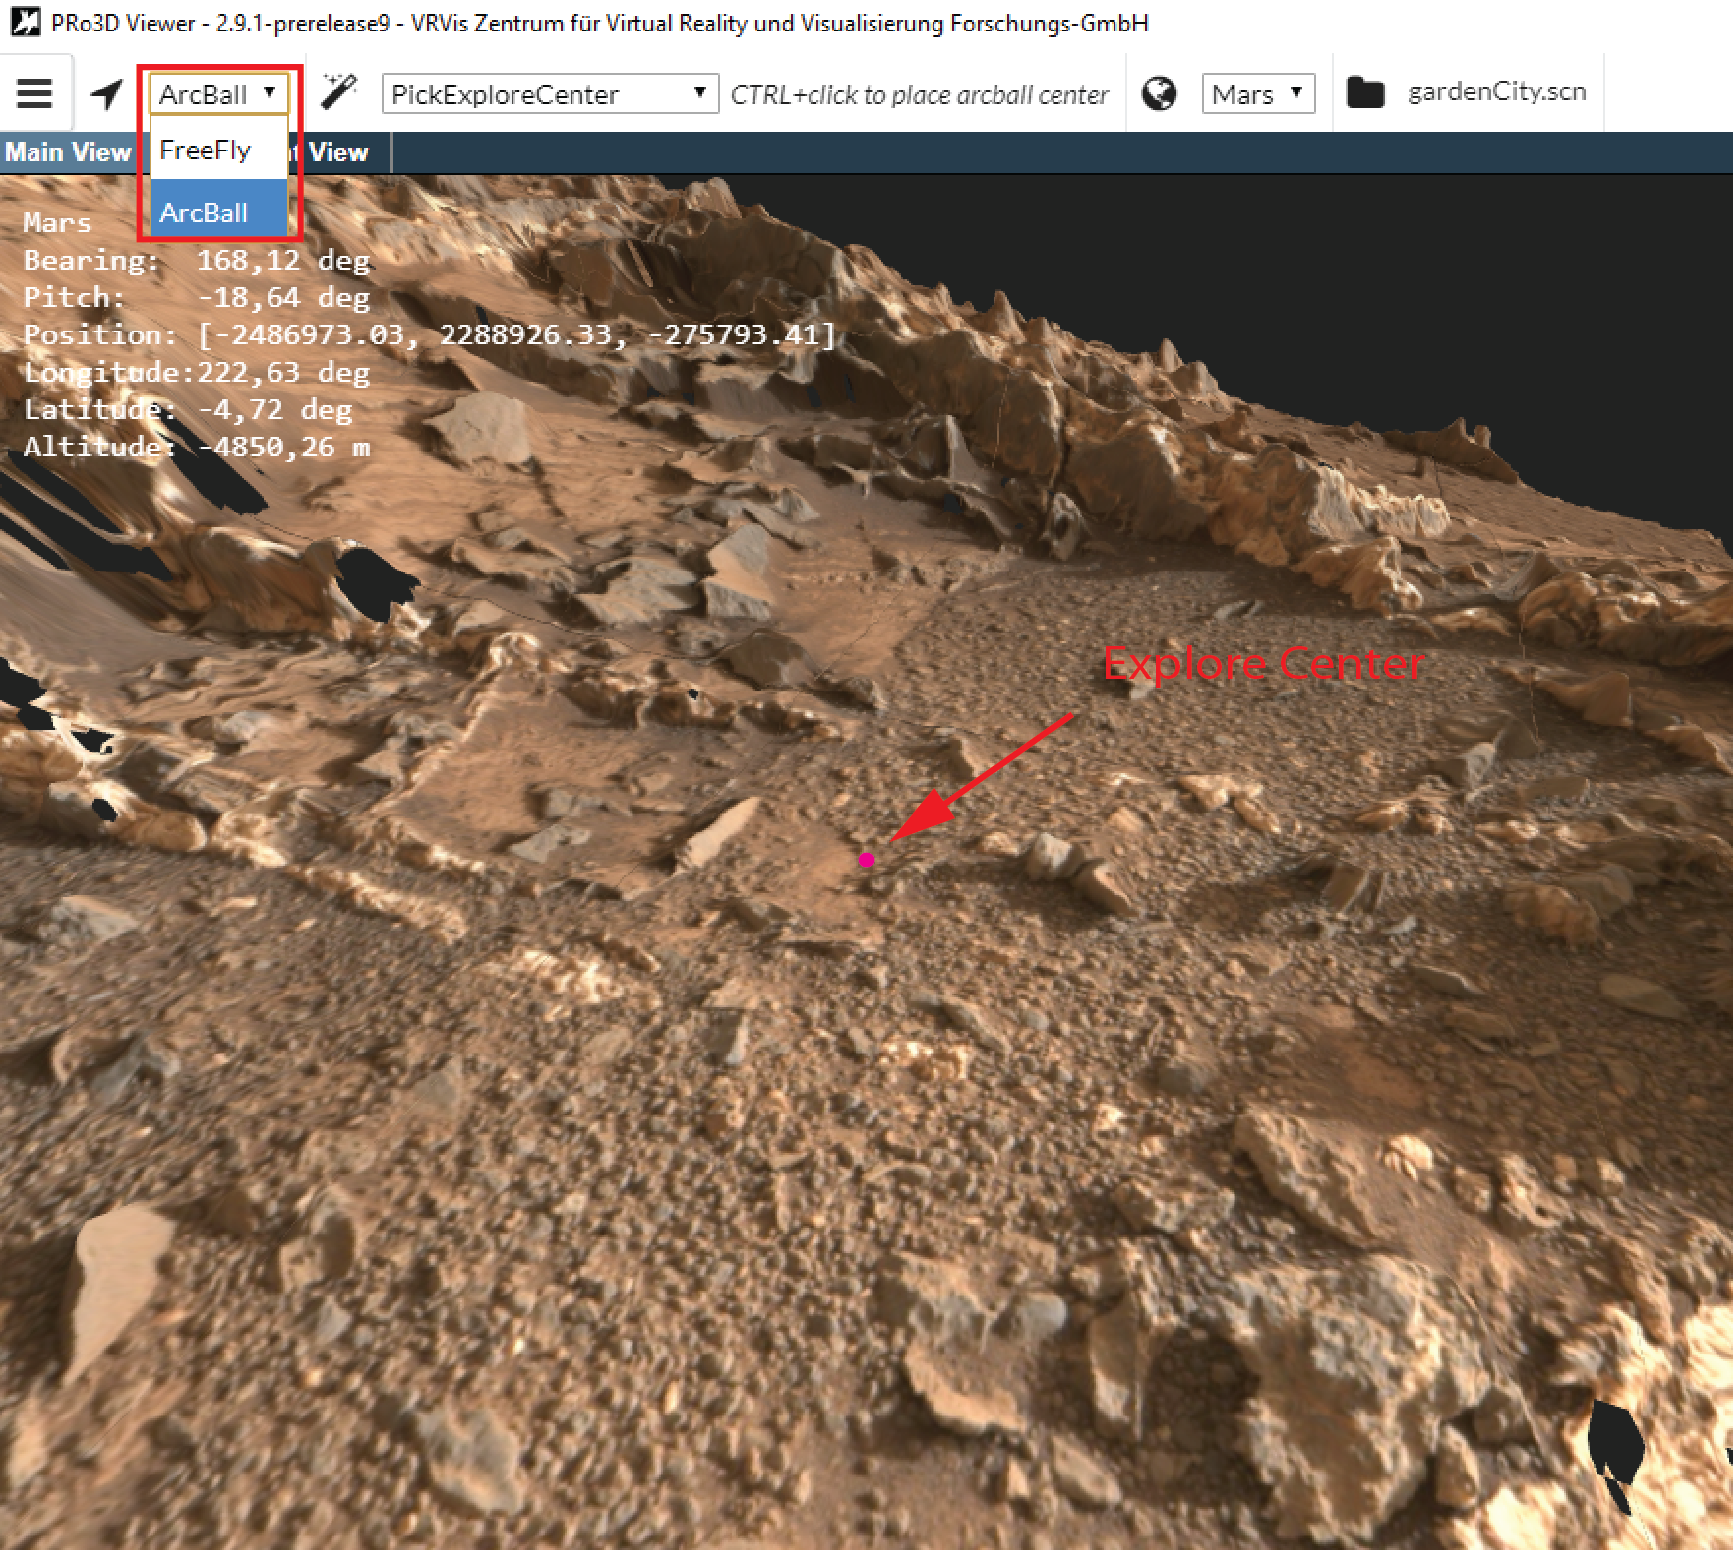
\includegraphics[width=1\textwidth]{pics/exploreCenterAI.png}
    	\caption[ExploreCenter]{ArcBall navigation. Explore center is set with CTRL + LMB and indicated by a pink dot.}
    	\label{fig:exploreCenter}
   \end{figure}

%----------------------------------------------------------------------------------------Free Fly-
\subsubsection{FreeFly}

The Free Fly Mode is the standard 3D fly-through navigation, as for instance, in terrain visualization. WASD controls forward/backward and strafing movement, while the user can change the camera's orientation by holding the LMB (= \textbf{L}eft \textbf{M}ouse \textbf{B}utton). Zooming in and out (forward/backward movement) is performed by turning the mouse-wheel or holding down the RMB (= \textbf{R}ight \textbf{M}ouse \textbf{B}utton). Additionally, the camera can be panned by holding down the middle mouse button.

%----------------------------------------------------------------------------------------Arc Ball-
\subsubsection{ArcBall}

When the viewer is in ArcBall mode the camera can be rotated around the explore center by holding down the LMB. Panning and strafing are possible as described above, but be aware that this moves the explore center (otherwise panning would break the view matrix of the camera). To set a new explore point, make sure the ``PickExploreCenter'' action is active (as shown in Figure~\ref{fig:exploreCenter}) and press CTRL + LMB on the surface. The explore center is indicated by a pink dot. Forward and backward movement is performed either by the keys W/S, rotating the mouse wheel, or clicking the RMB.
%----------------------------------------------------------------------------------------
%	SubSection: Place Coordinate System
%----------------------------------------------------------------------------------------
\subsection{Place Coordinate System}
\label{sec:placeCS}

\begin{figure}[h]
    	\centering
    		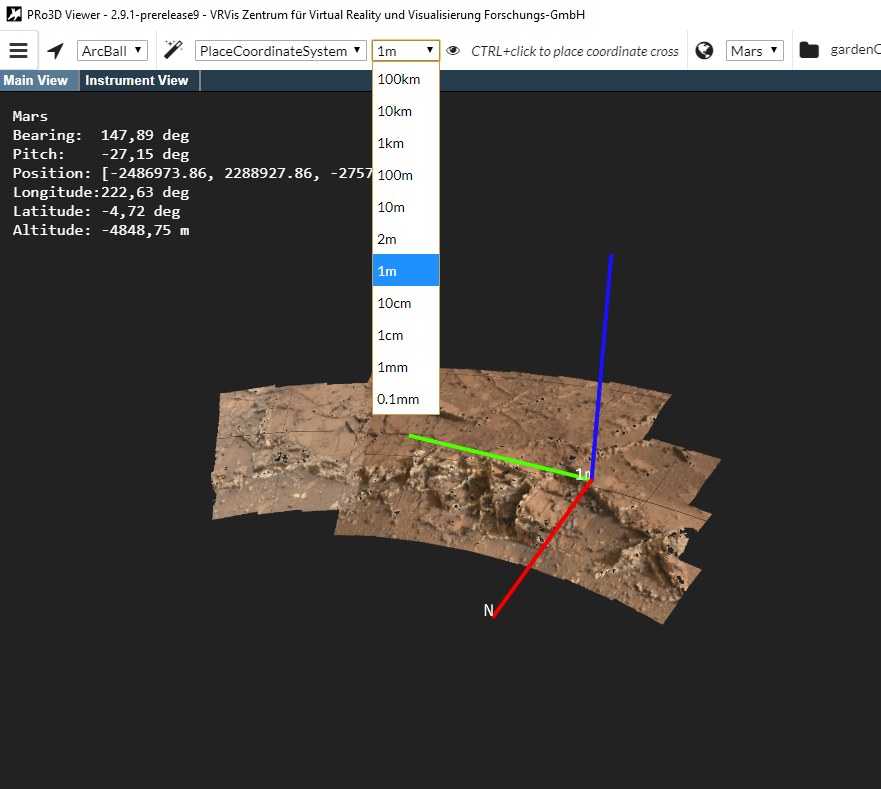
\includegraphics[width=1\textwidth]{pics/CoordinateSystem.png}
    	\caption[Coordinate System]{Coordinate System with scale bar functionality.}
    	\label{fig:coordinateSystem}
   \end{figure}
	
To set the coordinate system pick ``PlaceCoordinateSystem'' in the actions drop down menu, select a unit of measurement and press CTRL+LMB to pick a point on the surface. This marks the position as shown in Figure~\ref{fig:coordinateSystem}.
Initially the up vector's (blue) direction is set in the positive z-direction and the north vector's (red) in the positive y-direction. You can manipulate the north vector manually for different data. The surface can be translated along the three directions of the coordinate system, as described in Section~\ref{sec:surfaces}. The up- and the north vector are used for the projection measurements. The north vector is also relevant for bearing measurements, and the rover placement in the View Planner.
%(see Section~\ref{sec:viewPlanner})
The value for manipulating the north vector is shown in the Viewer Configuration described in Section~\ref{sec:config}.
%----------------------------------------------------------------------------------------
%	SubSection: Draw Annotation
%----------------------------------------------------------------------------------------
\subsection{Draw Annotation}
\label{sec:drawAnnotation}

\begin{figure}[h]
    	\centering
    		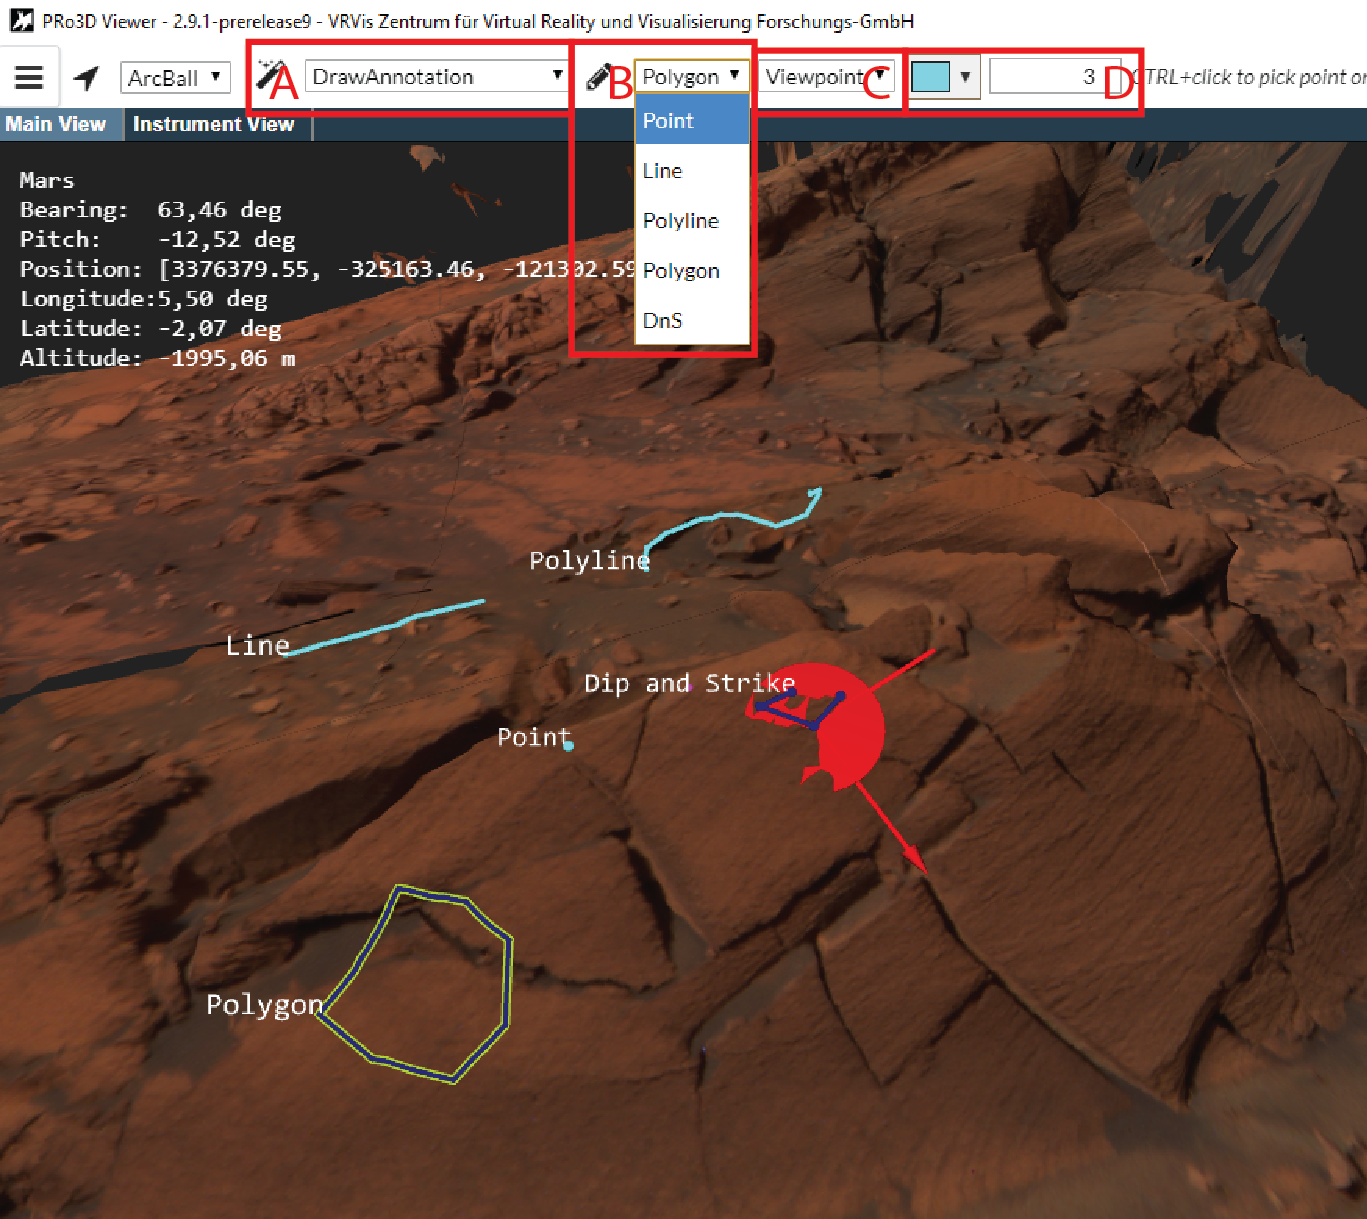
\includegraphics[width=1\textwidth]{pics/drawAnnotationsAI.png}
    	\caption[Draw Annotations]{Annotation settings: \textbf{A}: set viewer action to ``DrawAnnotation. \textbf{B}: select annotation mode. \textbf{C}: select projection. \textbf{D}: choose color and thickness. }
    	\label{fig:drawAnnotations}
   \end{figure}
	
Figure~\ref{fig:drawAnnotations} shows the settings for drawing annotations. First set ``DrawAnnotation'' in the actions menu (A in Figure~\ref{fig:drawAnnotations}). Then you can choose one of the following annotation modes (B in Figure~\ref{fig:drawAnnotations}):
\begin{itemize}
	\item \textit{Point}: A single point measurement on the surface.
	\item \textit{Line}: You can pick two points on the surface. The connecting line depends on the projection mode explained in the table below.
	\item \textit{Polyline}: An arbitrary number of points on the surface can be picked. The connecting line segments depend on the projection mode. The polyline is finished by pressing Enter.
	\item \textit{Polygon}: An arbitrary number of points on the surface can be picked. The connecting line segments depend on the projection mode. The region of interest is closed and finished by pressing Enter.
	\item \textit{DnS}: (\textit{= Dip and Strike}) A polyline onto a surface, e.g. alongside a rock layer can be picked. After clicking Enter, a plane is fitted (least squares) to this polyline (blue), which is then intersected with a horizontal plane, which gives us the so-called strike vector (red). This vector represents the direction within the plane with the least inclination and orthogonal to it is the dip vector (green) which shows the direction of highest inclination as shown in Figure~\ref{fig:drawAnnotations}.
\end{itemize}
To pick an annotation point on the surface press CTRL+LMB.

For all annotations (except Point) you can choose between ``Linear'', ``ViewPoint'' and ``Sky'' projection which determines the direction of the picking ray (C in Figure~\ref{fig:drawAnnotations}):
\begin{itemize}
	\item \textit{Linear}: produces straight line segments as point-to-point connections with linear interpolation between them, no actual projection is performed (Figure~\ref{fig:projection}, blue line). This is useful for line-of-flight distance measurements or measuring the height of a cliff or determining its slope.
	\item \textit{ViewPoint}: between two points we sample the space by shooting additional rays to intersect with the surface, in this case along the view direction (Figure~\ref{fig:projection}, green line). This is helpful to measure details in nooks and crannies of a rough surface and is the typical way to go for geological measurements.
	\item \textit{Sky}: the same sampling happens as for the viewpoint projection but this time the rays are shot along the scene's up-vector (Figure~\ref{fig:projection}, pink line). This mode is useful for geographical measurements to estimate the length of a path through a crater.
\end{itemize}

\begin{figure}[h]
    	\centering
    		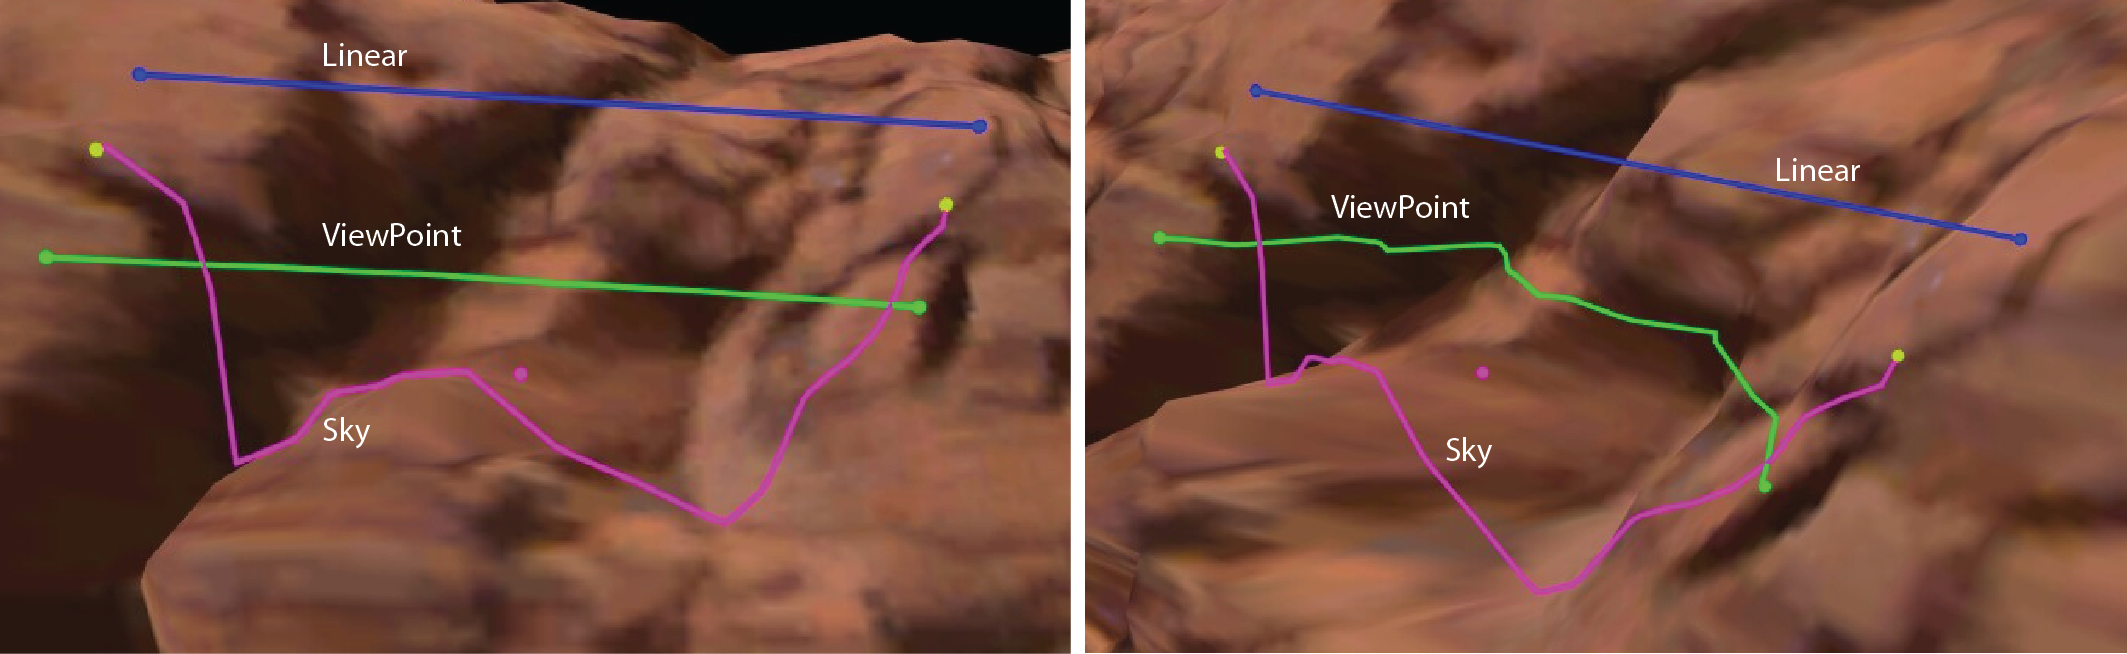
\includegraphics[width=1\textwidth]{pics/projectionAI.png}
    	\caption[Projections]{Three Lines taken from the same camera position (left) with the same camera settings but with different line projections.}
    	\label{fig:projection}
   \end{figure}
	
Finally you can set the color and thickness of the annotation (D in Figure~\ref{fig:drawAnnotations}).
Section~\ref{sec:annotations} shows how to maintain, group and edit existing annotations.

%----------------------------------------------------------------------------------------
%	SubSection: Pick Annotation
%----------------------------------------------------------------------------------------
\subsection{Pick Annotation}
\label{sec:pickAnnotation}

There are two ways to select an annotation:

\begin{enumerate}
	\item You can select an annotation by clicking on the annotation's name in the annotation's listing described in Section~\ref{sec:annotations}.
	\item Or you set ``PickAnnotation'' in the actions menu, press CTRL+LMB and pick the annotation in the main view.
\end{enumerate}
Then the annotation turns its color to green in the listing and gets a green border in the main view as shown in Figure~\ref{fig:drawAnnotations}, where the Polygon is selected. Once selected, you can explore and adjust the annotation's properties (see Section~\ref{sec:annotations}).
%----------------------------------------------------------------------------------------
%	SubSection: Pick Surface
%----------------------------------------------------------------------------------------
\subsection{Pick Surface}
\label{sec:pickSurface}

There are two ways to select a surface:

\begin{enumerate}
	\item You can select a surface by clicking on the surface's name in the surface's listing described in Section~\ref{sec:surfaces}.
	\item Or you set ``PickSurface'' in the actions menu, press CTRL+LMB and pick the surface in the main view.
\end{enumerate}
Then the surface's name turns its color to green in the listing. Once selected, you can explore and adjust the surface's properties (see Section~\ref{sec:surfaces}).

%----------------------------------------------------------------------------------------
%	SubSection: Place Rover
%----------------------------------------------------------------------------------------
%\subsection{Place Rover}
%\label{sec:placeRover}

%----------------------------------------------------------------------------------------
%	SubSection: Trafo Controls
%----------------------------------------------------------------------------------------
%\subsection{Trafo Controls}
%\label{sec:trafoControls}

%----------------------------------------------------------------------------------------
%	SubSection: Align Pick
%----------------------------------------------------------------------------------------
%\subsection{Align Pick}
%\label{sec:alignPick}

